\section{Software in the Loop}

\subsection{Monte-Carlo}

\section{Hardware in the Loop}

\clearpage
\section{Testflight}
The Testflight launch was conducted on May 10th 2025 near Louisville, Kentucky.
Due to an error with internal logging only the telemetry data is available. This data was transmitted by the Processor Board to the rocket CAN bus, sent over radio telemetry, and logged by the ground station computer.
The resulting state estimation data is shown in Figure \ref{fig:testflight}.

Due to a safety lockout triggered by a timer, the canard was commanded to zero for the entirety of the flight.
Therefore the rocket had no control authority, and some misalignment of the canards and fin cant led to a slow roll rate with a peak of about 2 rad/s, as can be seen in Figure \ref{fig:testflight-w}.

\begin{figure}[ht]
    \centering   
    \begin{subfigure}{0.45\textwidth}
        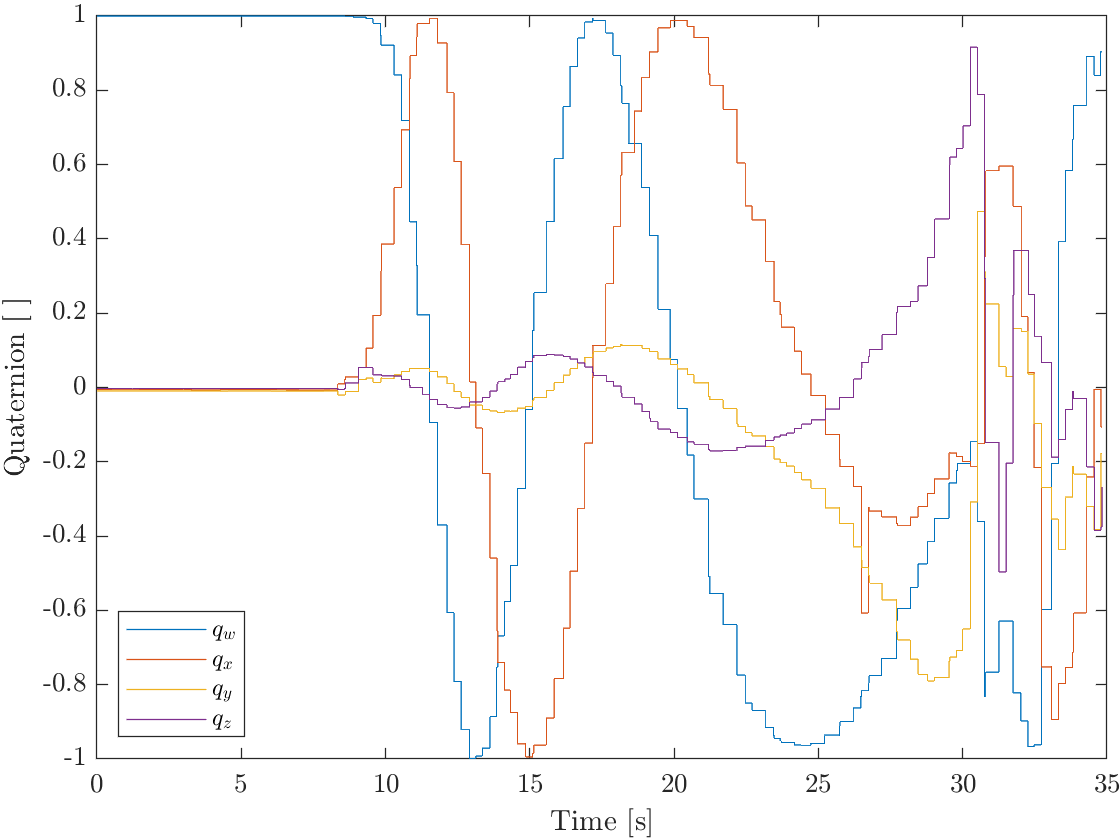
\includegraphics[width=0.95\textwidth]{images-results/testflight_q.png}
        \caption{Attitude Quaternion}
        \label{fig:testflight-q}
    \end{subfigure}
    \begin{subfigure}{0.45\textwidth}
        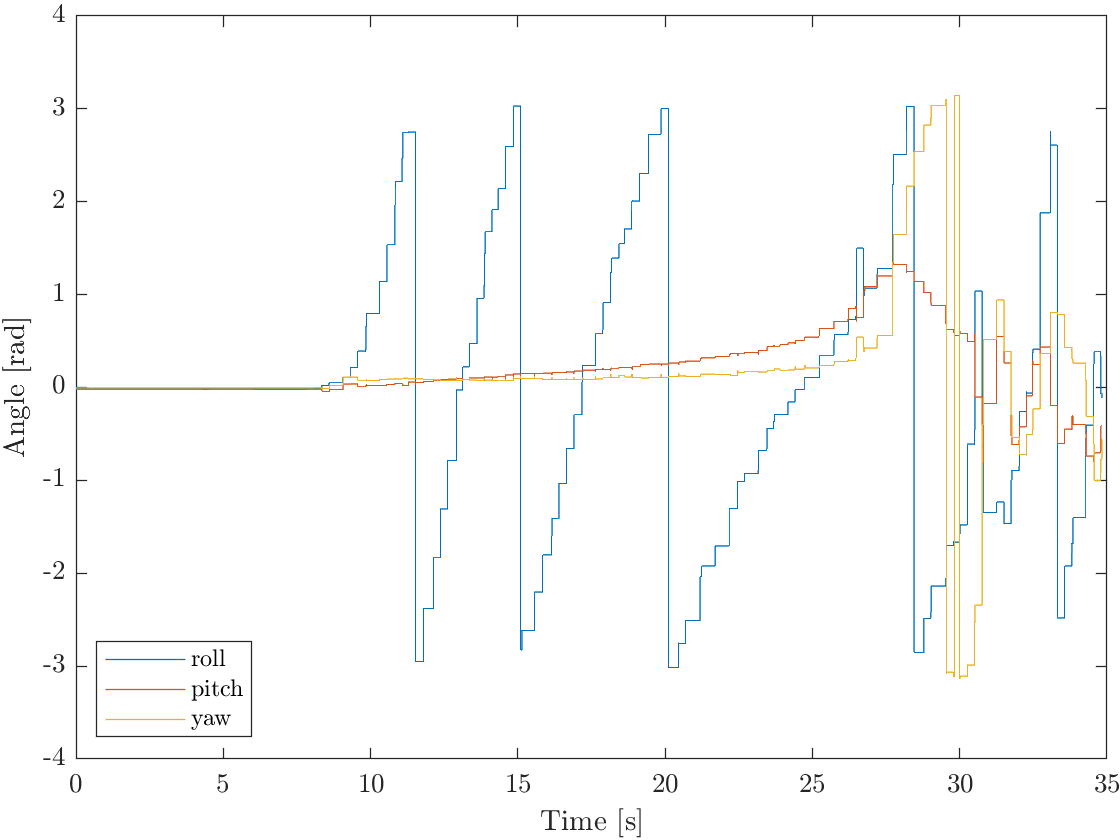
\includegraphics[width=0.95\textwidth]{images-results/testflight_euler.png}
        \caption{Attitude Euler angles}
        \label{fig:testflight-euler}
    \end{subfigure}
    \begin{subfigure}{0.45\textwidth}
        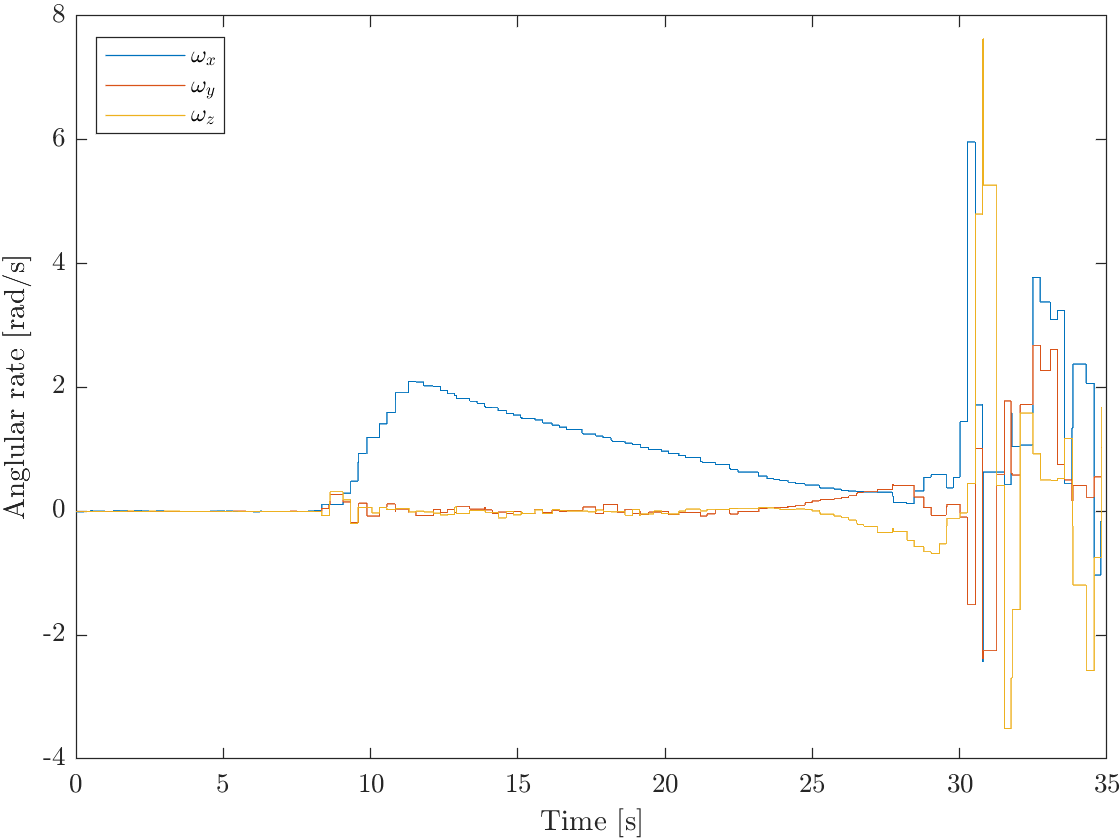
\includegraphics[width=0.95\textwidth]{images-results/testflight_w.png}
        \caption{Angular rates}
        \label{fig:testflight-w}
    \end{subfigure}
    \begin{subfigure}{0.45\textwidth}
        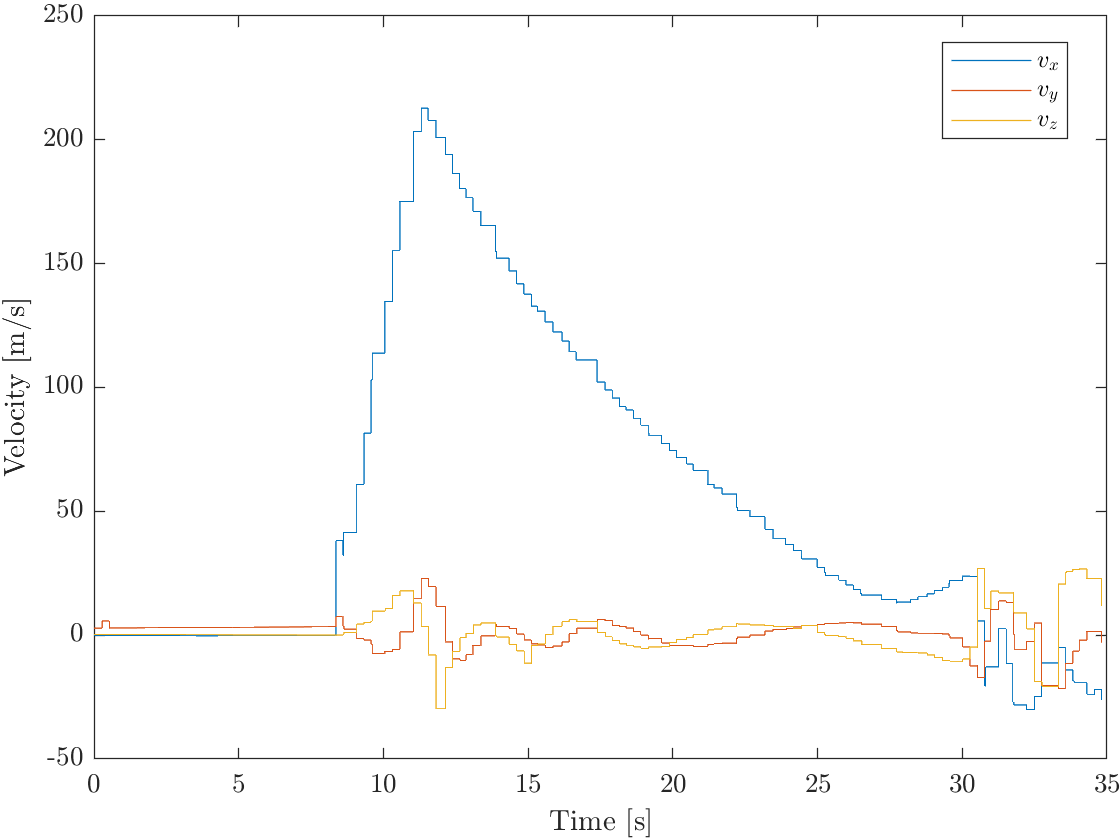
\includegraphics[width=0.95\textwidth]{images-results/testflight_v.png}
        \caption{Body velocity}
        \label{fig:testflight-v}
    \end{subfigure}
    \begin{subfigure}{0.45\textwidth}
        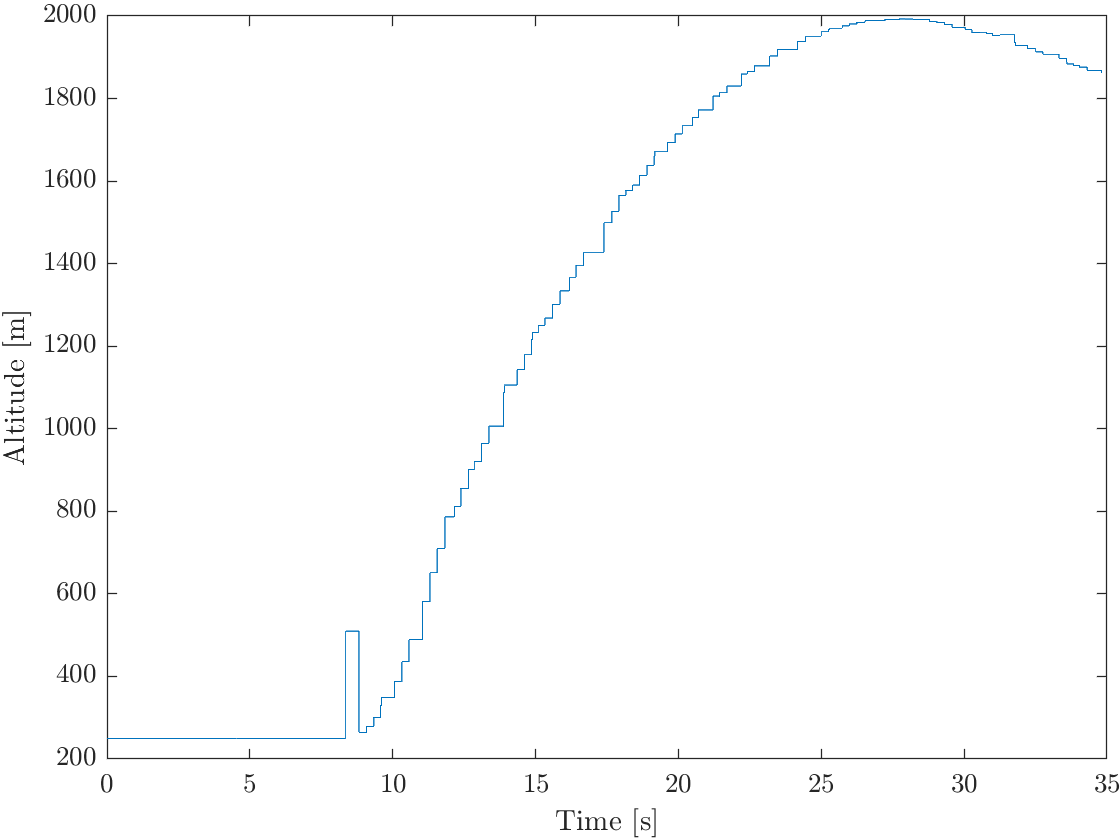
\includegraphics[width=0.95\textwidth]{images-results/testflight_alt.png}
        \caption{Altitude}
        \label{fig:testflight-alt}
    \end{subfigure}
    \begin{subfigure}{0.45\textwidth}
        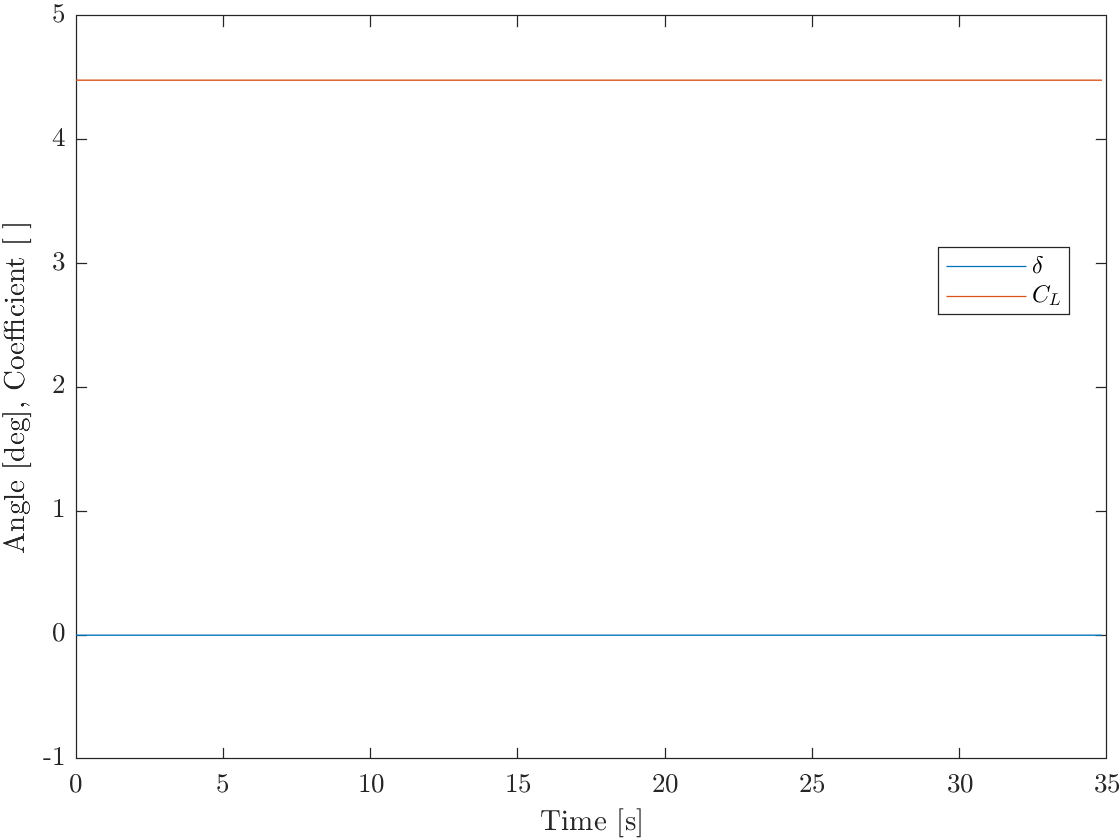
\includegraphics[width=0.95\textwidth]{images-results/testflight_canard.png}
        \caption{Canard}
        \label{fig:testflight-canard}
    \end{subfigure}
    \caption{Testflight telemtry, estimated state}
    \label{fig:testflight}
\end{figure}

\clearpage
\section{Competition flight}
